% ----------------------------------------------------------------------------------------------------------------------------------
% Reviewing PostgreSQL Patches for Fun and Profit
%
% Build from the Vagrant VM:
% cd /talk/slides && make -f /template/Makefile
% ----------------------------------------------------------------------------------------------------------------------------------
\def\mytitle{Reviewing PostgreSQL Patches for Fun and Profit}
\def\mysubject{}
\def\myevent{PGConf.EU 2016}
\def\myauthor{David Steele}
\def\myemail{}
\def\mydate{November 2, 2016}

% Suppres navigation bars
\def\mysuppressnav{}

% Include Crunchy template
\def\mytemplatepath{/template/}
\input{\mytemplatepath crunchy-template.tex}

%-----------------------------------------------------------------------------------------------------------------------------------
\section{Introduction}

\begin{frame}
    \frametitle{The Goal}

    \large How can we economize committer time?
\end{frame}

\begin{frame}
    \frametitle{The Purpose of Patch Review}

    The purpose of patch review is to answer the following questions:

    \begin{itemize}
        \item Does the patch work as specified?\pause
        \item Is it useful and needed?\pause
        \item Does the functionality already exist?\pause
        \item Are documentation and tests included?\pause
        \item Does it follow applicable SQL or community standards?\pause
        \item Is performance acceptable?
    \end{itemize}
\end{frame}

\begin{frame}
    \frametitle{How can we help?}

    \begin{itemize}
        \item It is perfectly OK to only review parts of a patch, or only go through certain review steps.\pause

        \item PostgreSQL is a community project and all contributors have different strengths.  Some contributors might excel at documentation while others have a variety of platforms available for performance testing.\pause

        \item No contribution is too small, especially to start.
    \end{itemize}
\end{frame}

%-----------------------------------------------------------------------------------------------------------------------------------
\section{Selecting a Patch}

\begin{frame}
    \frametitle{The Commitfest App}

    \begin{itemize}
        \item Located at \url{https://commitfest.postgresql.org}
        \item Shows past, current, and future commitfests.
    \end{itemize}

    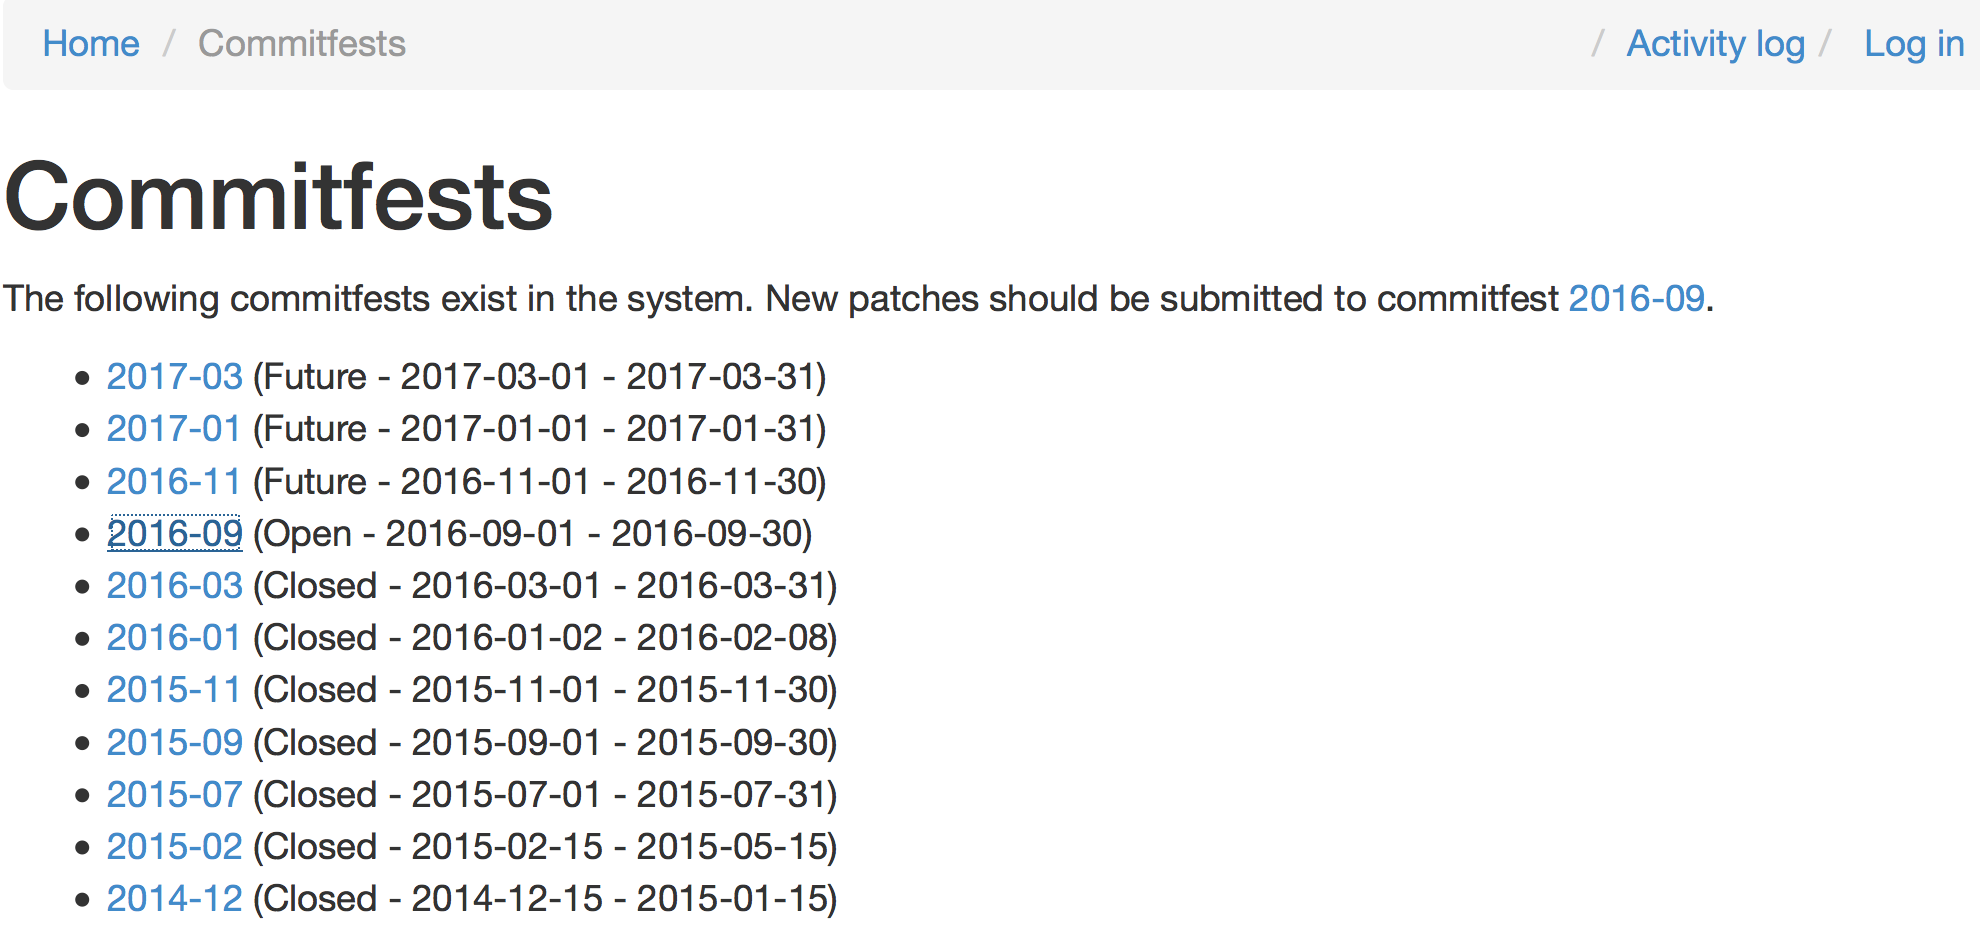
\includegraphics[width=10cm]{/talk/slides/images/cf-main.png}
\end{frame}

\begin{frame}
    \frametitle{The Commitfest App - Patch List}

    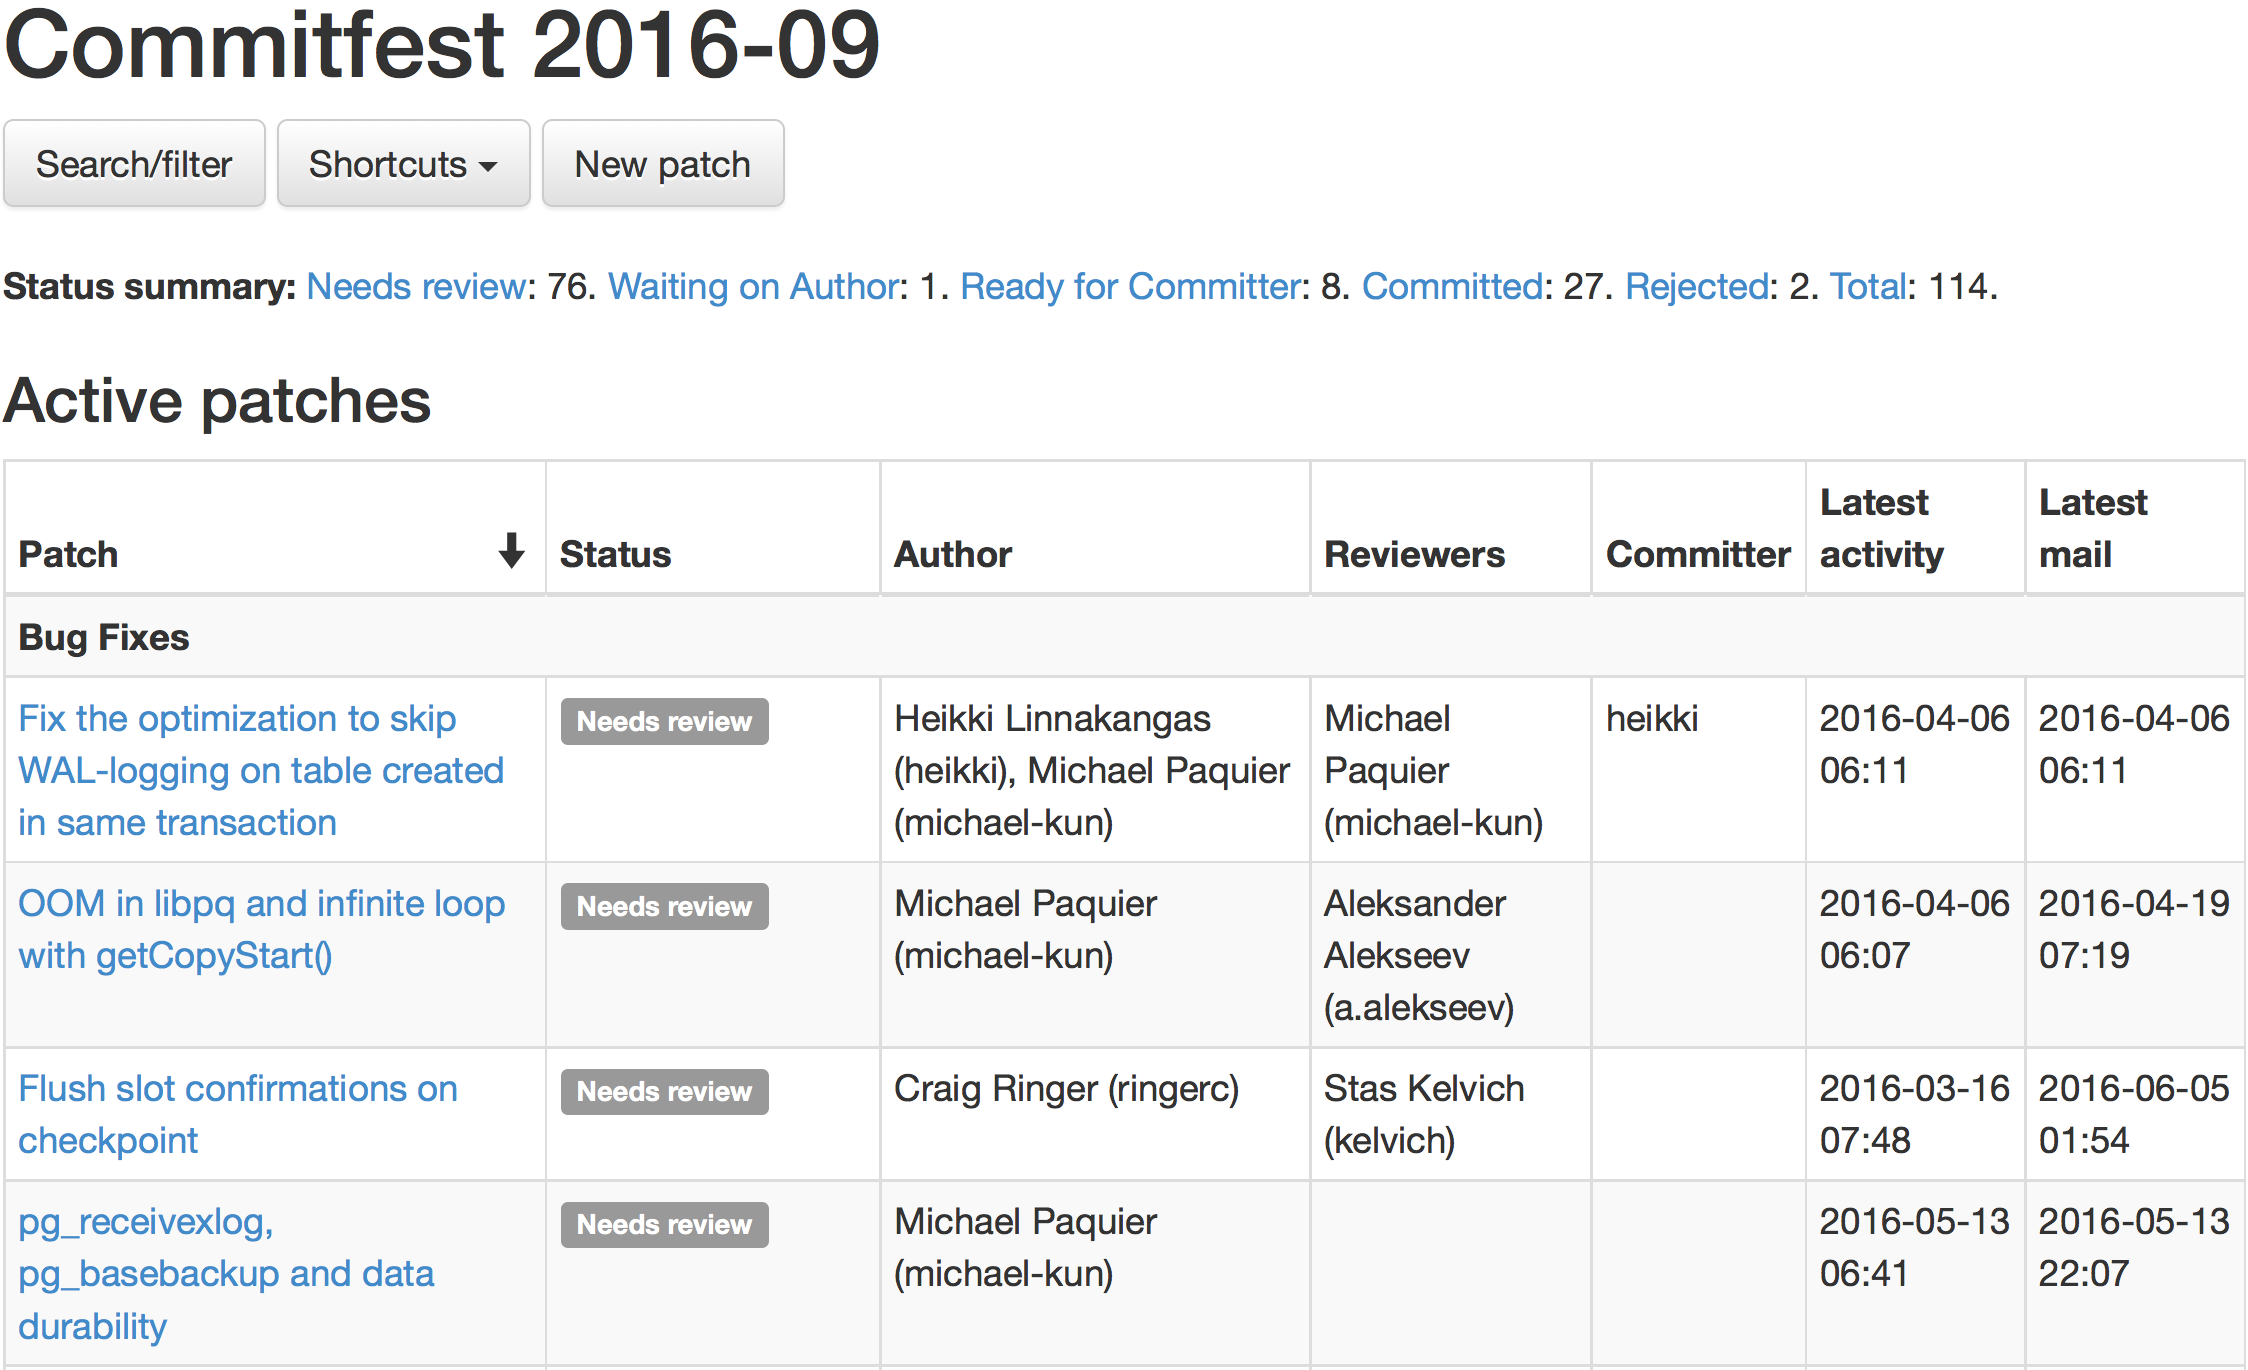
\includegraphics[width=12cm]{/talk/slides/images/cf-list.png}
\end{frame}

\begin{frame}
    \frametitle{The Commitfest App - Patch Information}

    \vspace{.5em}
    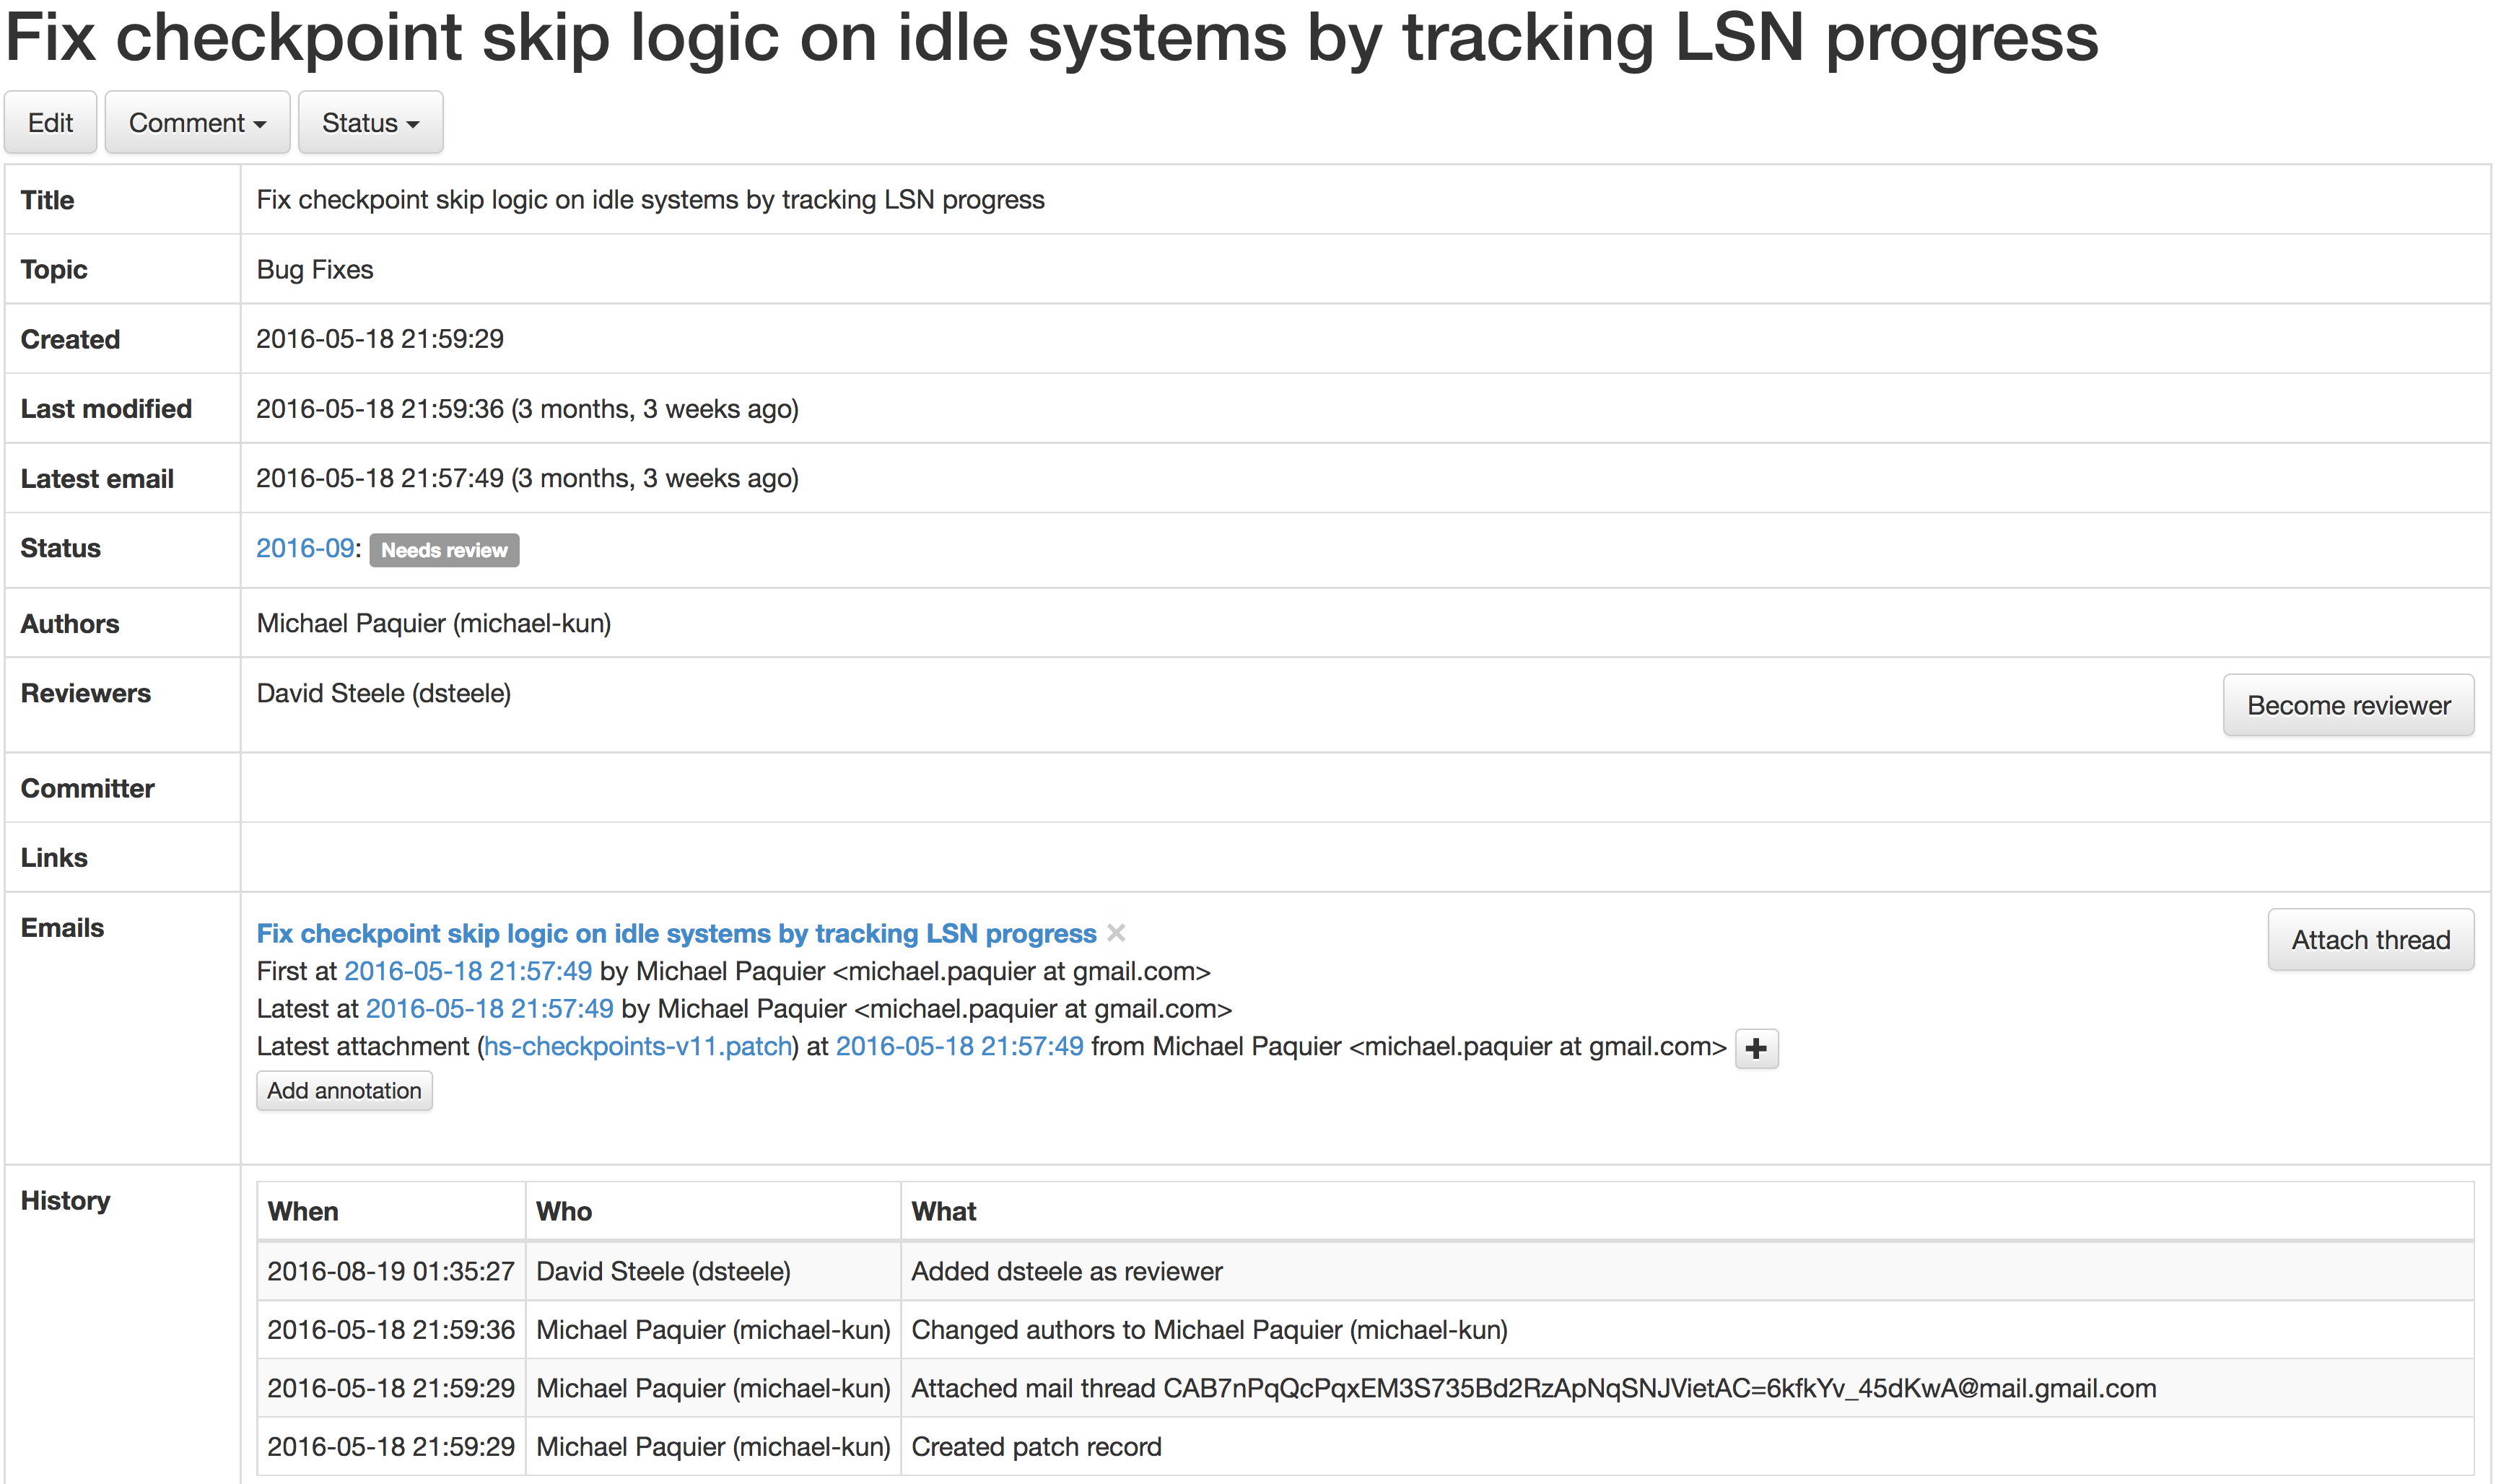
\includegraphics[width=12cm]{/talk/slides/images/cf-patch.png}
\end{frame}

\begin{frame}
    \frametitle{Patch Thread}

    All discussion about a patch is done on the pgsql-hackers mailing list:

    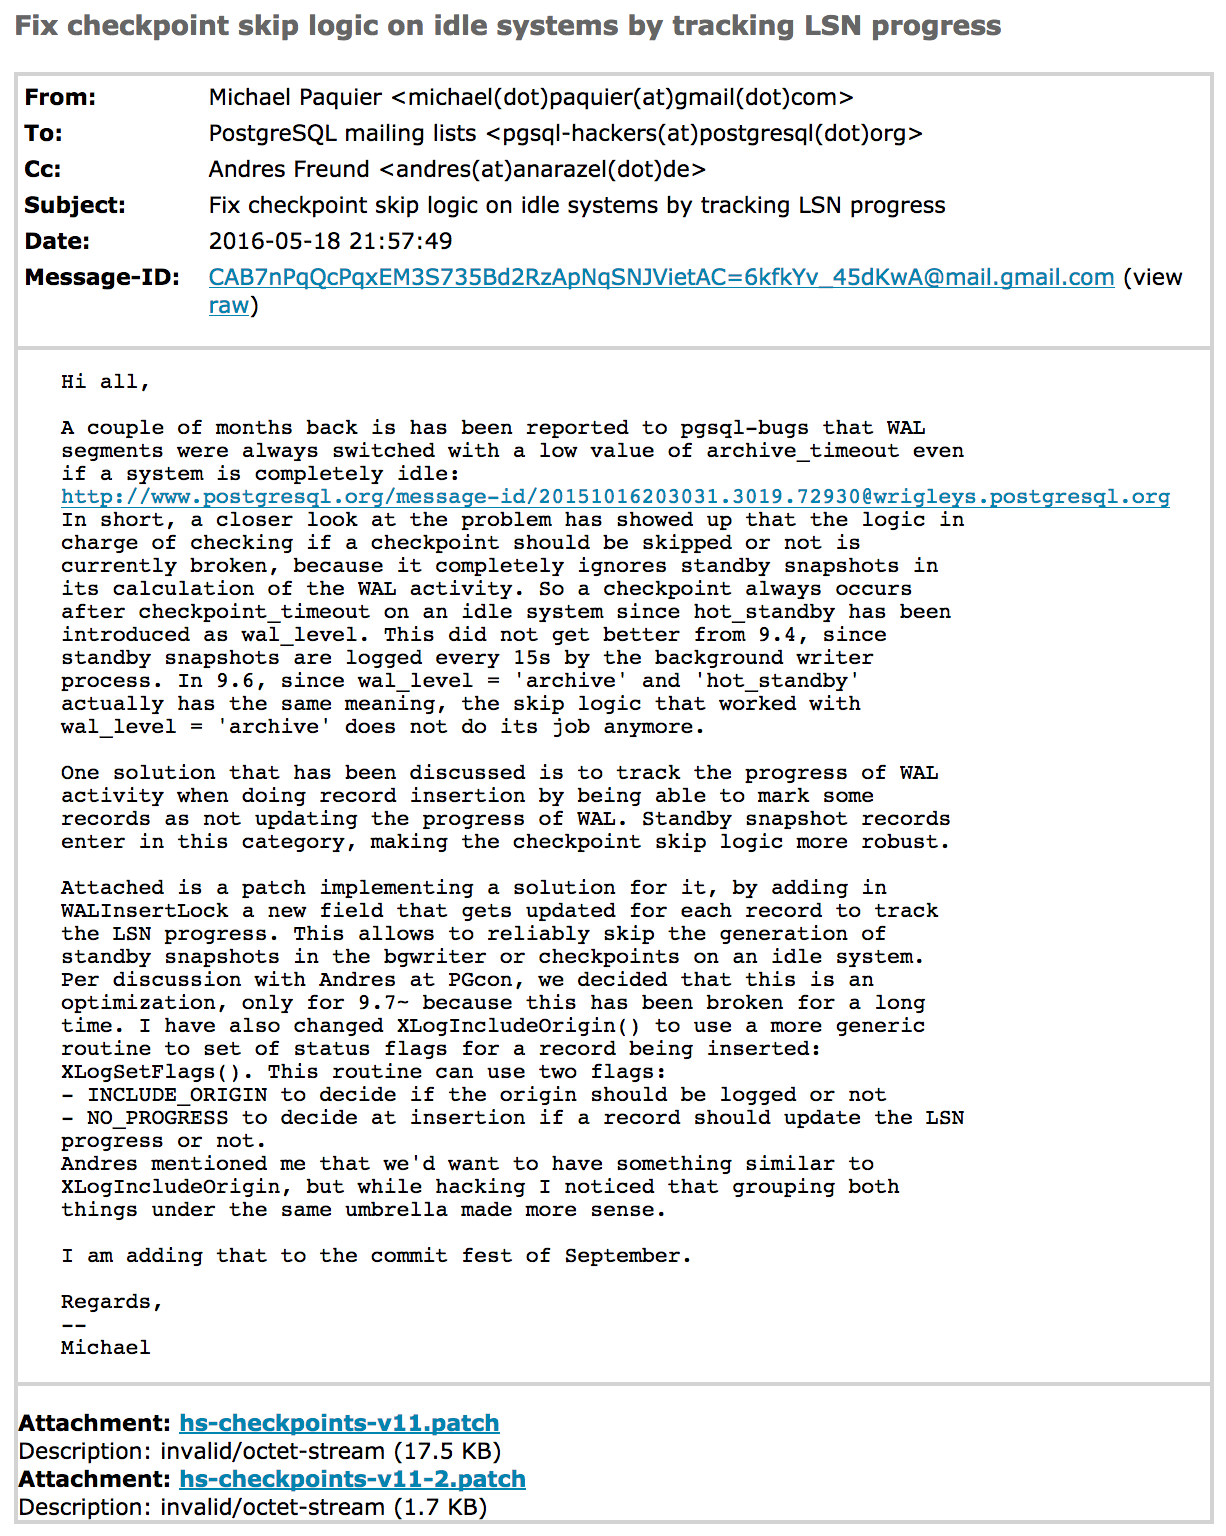
\includegraphics[height=7cm]{/talk/slides/images/cf-thread.png}
\end{frame}

\begin{frame}
    \frametitle{Patch Assessment}

    Read the entire thread relating to the patch.  Sometimes there will be more than one, but they should all be listed on the patch page.  Then ask:\pause

    \begin{itemize}
        \item Is there consensus on how this patch should work?\pause
        \item Have the details of this patch been finalized?\pause
        \item Has a patch been provided that addresses all concerns?\pause
    \end{itemize}

    If the answer to all these questions is yes, then proceed to review the patch.  Otherwise, try to determine what is holding the patch up:\pause

    \begin{itemize}
        \item Is the author waiting on a consensus?\pause
        \item Are there technical issues?\pause
        \item Anything you can do to help?
    \end{itemize}
\end{frame}

\begin{frame}
    \frametitle{Replying to a Thread}

    Reply to a thread by saving the raw message to a file (.eml) and then loading it into your email client.\pause

    \begin{itemize}
        \item Stay on topic\pause
        \item Be professional\pause
        \item Don't ``top post"\pause
    \end{itemize}

    Read the introduction to mailing lists (\url{https://wiki.postgresql.org/wiki/Mailing_Lists}).\pause\\
    \vspace{1em}
    Remember that your posts are visible to the public and archived indefinitely. See the archives policy (\url{https://wiki.postgresql.org/wiki/Archives_Policy}) for more information.
\end{frame}

%-----------------------------------------------------------------------------------------------------------------------------------
\section{Reviewing a Patch}

\begin{frame}
    \frametitle{Declare Your Intentions}

    \begin{itemize}
        \item Respond on the patch thread and declare which parts of the patch you are planning to review:

        \begin{itemize}
            \item Documentation, functional testing, performance analysis, etc.\pause
            \item Informs other potential reviewers of coverage so they can address different areas or move on to another patch.\pause
        \end{itemize}

        \item It is perfectly fine to have more than one person reviewing any given area.  A larger/complicated patch should have more reviewers while a small/simple patch can get by with one or two.\pause

        \item Remember, the committer will always review all aspects of the patch, but we would like to save them as much time as possible.
    \end{itemize}
\end{frame}

\begin{frame}[fragile]
    \frametitle{Documentation Review}

    PostgreSQL documentation is written in SGML. For example:
    \vspace{1em}

    \begin{lstlisting}
diff --git a/doc/src/sgml/backup.sgml b/doc/src/sgml/backup.sgml
index 7413666..9092cf8 100644
--- a/doc/src/sgml/backup.sgml
+++ b/doc/src/sgml/backup.sgml
@@ -592,7 +592,7 @@ <title>Setting Up WAL Archiving</title>

    <para>
     To enable WAL archiving, set the <xref linkend="guc-wal-level">
-    configuration parameter to <literal>archive</> or higher,
+    configuration parameter to <literal>replica</> or higher,
     <xref linkend="guc-archive-mode"> to <literal>on</>,
     and specify the shell command to use in the <xref
     linkend="guc-archive-command"> configuration parameter.  In practice
    \end{lstlisting}
    \vspace{1em}
    If the feature is user-facing then the SGML documentation should explain how it works.  If the feature is only exposed internally then there may not be any SGML documentation but there should still be code comments and an explanation in the email thread.
\end{frame}

\begin{frame}[fragile]
    \frametitle{Documentation Review - Continued}

    \begin{itemize}
        \item Documentation is an excellent area for non-coders to contribute.  It can be difficult for patch authors to write good user-facing documentation and they appreciate another take on how to best explain a feature.\pause

        \item In addition, many patch authors are not native English speakers.  If you are fluent don't be afraid to fix grammatical mistakes or clean up awkward phrasing.\pause

        \item Look for areas where a potential user of the feature may misunderstand the intent.  Clarify where possible while keeping the documentation concise.
    \end{itemize}
\end{frame}

\begin{frame}[fragile]
    \frametitle{Apply and Compile the Patch}

    Compiling PostgreSQL after applying a patch is another area for non-coders to contribute.
    \vspace{1em}

    \begin{lstlisting}
git clone git://git.postgresql.org/git/postgresql.git
cd postgresql
./configure

git apply ../basebackup-exclusions-v3.patch
make install
    \end{lstlisting}
\end{frame}

\begin{frame}
    \frametitle{Patch Does Not Apply/Compile}

    \begin{itemize}
        \item It is not uncommon for a patch to get out of date during a commitfest when many other patches are being committed to master.  If the patch does not apply or compile on HEAD (i.e., the most recent commit in the master branch) then try to determine the cause of the issue.\pause

        \item If the patch does not apply/compile on HEAD then try to find a commit in master where it does apply/compile.  Do this by picking a commit that is close to the date that the patch was originally posted, as it may be later changes in master that are causing the problem.\pause

        \item Sometimes the patch author will specify a commit that is known to work in the email thread.  If no commit can be found where the patch applies/compiles then reply on the patch thread with the error message you are receiving and the commits that were tested.
    \end{itemize}
\end{frame}

\begin{frame}
    \frametitle{Test Functionality}

    \begin{itemize}
        \item Functional testing requires a working knowledge of PostgreSQL but no coding experience.\pause

        \item Test the patch and make sure that it does what is specified in the SGML documentation and/or the email thread.  If there is a discrepancy then it may indicate an error in either the code or the documentation.\pause

        \item You can either suggest a fix or simply report the issue on the email thread.
    \end{itemize}
\end{frame}

\begin{frame}
    \frametitle{Performance Testing}

    \begin{itemize}
        \item The new feature should have acceptable performance (though this is somewhat subjective).\pause

        \item More importantly, the new feature should not cause a performance regression in an existing feature without good reason.\pause

        \item Performance testing is often done by developers with access to unique/large scale systems.
    \end{itemize}
\end{frame}

\begin{frame}
    \frametitle{Code Review}

    \begin{itemize}
        \item Final code review is the last step and should generally be undertaken by coders experienced in the language and conversant with the project coding standards.\pause

        \item However, the doesn't mean that less experienced coders can't jump in and try to figure out what is going on, especially when the patch does not apply/compile or functional testing fails.  Any information you can give the authors is appreciated.\pause

        \item Also, the best way to learn how to do a good review is to give it a try and see what kind of feedback you get.  Over time this feedback will lead to greater confidence and ability.
    \end{itemize}
\end{frame}

%-----------------------------------------------------------------------------------------------------------------------------------
\section{Questions?}

\begin{frame}
    \frametitle{Questions?}

    website: \url{http://www.crunchydata.com}\\
    \vspace{1em}
    email: \href{mailto:david@crunchydata.com}{david@crunchydata.com}\\
    \vspace{1em}
    slides \& demo: \url{https://github.com/dwsteele/conference/releases}\\
\end{frame}

\end{document}
